\documentclass[a4paper,12pt,twosided]{report}
\usepackage[utf8]{inputenc}
\usepackage{datetime}
\usepackage{url}
\usepackage[pdftex]{graphicx}
\usepackage{epstopdf}
\usepackage{amsmath}
\usepackage{mathtools}
\usepackage{listings}
\usepackage{float}
\usepackage{subcaption}

% Bibliography
\usepackage[nottoc]{tocbibind}
\usepackage[square]{natbib}
\renewcommand\cite{\citep}

% Chart plotting
\usepackage{tikz}
\usepackage{pgfplots}
\usetikzlibrary{matrix,snakes,patterns}
\usetikzlibrary{decorations.pathmorphing}
\usetikzlibrary{decorations.markings}
\usetikzlibrary{plotmarks}
\tikzstyle{inChart}=[anchor=north east]
\tikzstyle{grid}=[loosely dotted] % [ultra thin] % % [dotted]
\newcommand{\subt}[3] { 
  \draw[grid] (#1,#1) -- (#1,#2) node[inChart] {#3} -- (#2,#2);
  \fill[color=black] (#1,#2) circle (2pt)
 }
\newcommand{\mrk}[2]{\node[inChart] at (#1,#1) {#2}}

% Haskell (and other) source code listing
\usepackage{listings}
\lstloadlanguages{Haskell}
\lstnewenvironment{code}
    {\lstset{}%
      \csname lst@SetFirstLabel\endcsname}
    {\csname lst@SaveFirstLabel\endcsname}
    \lstset{
      basicstyle=\small\ttfamily,
      numbers=left,
      frame=single,
      flexiblecolumns=false,
      basewidth={0.5em,0.45em},
      literate={+}{{$+$}}1 {/}{{$/$}}1 {*}{{$*$}}1 {=}{{$=$}}1
               {>}{{$>$}}1 {<}{{$<$}}1 {\\}{{$\lambda$}}1
               {\\\\}{{\char`\\\char`\\}}1
               {->}{{$\rightarrow$}}2 {>=}{{$\geq$}}2 {<-}{{$\leftarrow$}}2
               {<=}{{$\leq$}}2 {=>}{{$\Rightarrow$}}2 
               {\ .}{{$\circ$}}2 {\ .\ }{{$\circ$}}2
               {>>}{{>>}}2 {>>=}{{>>=}}2
               {|}{{$\mid$}}1               
    }

\newdateformat{monthdate}{\monthname[\THEMONTH] \THEYEAR}

\begin{document}
% Adapted the GU template from word to LaTeX
\begin{titlepage}
\thispagestyle{empty}

\begin{center}

\includegraphics[width=\textwidth]{gulogo.pdf}
\end{center}

% TODO: Find a good cover photo, perhaps the result from some generated matrix?
% \includegraphics[width=0.5\textwidth]{cover.pdf}

\vfill

\begin{flushleft}
{\LARGE Implementing incremental and parallel parsing} \\[0.2cm]
{\large \textit{Master of Science Thesis in Computer Science}}\\[3cm]

{\Huge \textsc{Tobias Olausson}}

\vfill

University of Gothenburg \\
Chalmers University of Technology \\
Department of Computer Science and Engineering \\
Göteborg, Sweden, \monthdate\today
\end{flushleft}

\newpage
\thispagestyle{empty}

\noindent The Author grants to Chalmers University of Technology and University
of Gothenburg  the non-exclusive right to publish the Work electronically and in
a non-commercial purpose make it accessible on the Internet.  The Author
warrants that he is the author to the Work, and warrants that the Work does
not contain text, pictures or other material that violates copyright law.\\

\noindent The Author shall, when transferring the rights of the Work to a third
party (for example a publisher or a company), acknowledge the third party about
this agreement. If the Author has signed a copyright agreement with a third
party regarding the Work, the Author warrants hereby that he has obtained
any necessary permission from this third party to let Chalmers University of
Technology and University of Gothenburg  store the Work electronically and make
it accessible on the Internet. \\[2cm]

\noindent \textbf{Implementing incremental and parallel parsing}\\
\noindent \textsc{Tobias Olausson} \\

\noindent \copyright \textsc{ Tobias Olausson}, \monthdate\today \\

\noindent Examiner: \textsc{Patrik Jansson} \\

\noindent University of Gothenburg \\
Chalmers University of Technology \\
Department of Computer Science and Engineering \\
SE-412 96 Göteborg \\
Sweden \\
Telephone + 46 (0)31-772 1000 \\

\vfill

\noindent Department of Computer Science and Engineering \\
Göteborg, Sweden, \monthdate\today
\end{titlepage}


\begin{abstract}
Using recent improvements to Valiant's algorithm for parsing context-free
languages, We present an implementation of a generator of parsers that works
incrementally, that can be parallelized and generated from a grammar
specification. Using a tree structure makes for both easy use of incrementality
and parallelization.  The resulting code is reasonably fast and handles correct
input in a satisfactory way. It is however lacking important features such as
good error reporting.

TODO: Create a better abstract. Describe actual contribution to BNFC.
\end{abstract}

\tableofcontents

%
% NEW CHAPTER
%

\chapter{Background}

The topic of this thesis is to do \textbf{parsing} in an \textbf{incremental}
fashion that can easily be \textbf{parallelizable}, using a
\textbf{divide-and-conquer approach}. In this section, We will give a brief
explanation of the topics involved, and end with a motivation for why this is
interesting to do in the first place. Later in this chapter, the concept of
dependently typed programming will be discussed, because it is a vital technique
in the implementation of the parser.

\subsection{Divide-and-conquer}
Divide-and-conquer algorithms are a fundamental class of algorithms to computer
science. The name refers to the technique of breaking down a problem into
sub-problems, where the same rule is applied recursively (the divide step). Each
sub-problem can be solved independently, and the results of the sub-problems are
then combined, finally becoming the result of the initial problem (the conquer
step) \cite[p.209]{algorithmdesign}. A typical example is mergesort, where a
list of elements is broken down to lists of single elements (obviously sorted),
that are then combined using an improved insertion sort, observing that each
sub-list is sorted. It was shown by \citet{birdlists} that the conquer step has
to be associative, so that grouping of items does not effect the outcome of the
algorithm. 

Trees are a class of data structures that are especially suited for 
divide-and-conquer algorithms, because of their structure as trees with
subtrees, naturally following the divide-step. To conquer is just to reduce the
tree. It was shown by \citet{parparsepaper} that such a reduction can be made
for trees of symbols in a finite alphabet that is associative, thus preserving
the structure of the input. 

\subsection{Incrementality}
Doing something incrementally means that one does it step by step, and not
longer than neccessary. The concept has been used since the 70s
\cite{incrementalpaper}, but is especially relevant for code editor purposes,
where one typically only wants information about the snippet currently displayed
in the editor. For large files, this can save lots of work, so that rather than
parsing 1000 lines, one may only have to parse 50 of them. The text editor use
case has been described in more detail by Bernardy \cite{lazyfunctional} using
the Yi editor as subject. 

\subsection{Parallelism}
With computer architectures being parallel these days, with the ability to run
many threads simultaneosly, writing code that can be parallelized is crucial in
order to make use of these features, and thus having code that run physically in
parallel. Because divide-and-conquer algorithms usually work on several
independent sub-problems, they are well-suited for parallelization. For this to
become a reality, however, both the compiler and the source code must be written
in a special way to permit parallelization.

\subsection{Parsing}
To parse is to check if some given input corresponds to a certain language's
grammar, and in this thesis we will use \textbf{context-free grammars} for
programming languages. Many programming errors are syntactical ones, such as
misspelled keywords, missing parenthesis or semicolons and so on. All such
errors are caught in parsing. Parsing will be described in more detail in
section \ref{parsingsection}.

\subsection{Motivation}
In compilers, lexing and parsing are the two first phases. The output of these
is an abstract syntax tree (AST) which is fed to the next phase of the compiler.
An AST could also provide useful feedback for programmers, already in their
editor, if the code could be lexed and parsed fast enough. With a lexer and
parser that is incremental and that can also be parallelized, real-time feedback
in the form of an AST could easily be provided to the programmer. Most current
text editors give syntax feedback based on regular expressions, which does not
yield any information about, for example, nesting or the surrounding AST.  With a
fast incremental parser, one could also connect it to a type checker to get even
more information, possibly in real-time, while not having to recompile to get
such information.

\section{Lexing}
In compilers, a \textit{lexer} reads input source code and groups the characters
into sequences called \textit{lexemes} so that each lexeme has some meaning in
the language the compiler is built for \cite[p. 5, p. 109]{dragonbook}. The
lexemes are wrapped in \textit{tokens} that denote what function and position
each lexeme relates to. The tokens are then passed on to the parser for
syntactic analysis.

For a language like C, the code in figure \ref{lexsample} would be valid, and
can serve as an example of how lexing is done.  A lexer for C would recognise
that \texttt{while} is a keyword and place it in its own token. It would also
observe that \texttt{(}, \texttt{)}, \texttt{\{} and \texttt{\}} are used for
control grouping of code. Furthermore, \texttt{i} is an identifier and
\texttt{5} is a number, \texttt{$<$} and \texttt{++} are operators and
\texttt{;} denote separation of statements. All will be forwarded as tokens to
the parser.

\begin{figure}[H]
\begin{code}
while(i < 5) {
    i++;
}
\end{code}
\caption{A while loop that would be valid in C}
\label{lexsample}
\end{figure}

\subsection{LexGen}
A generator for incremental divide-and-conquer lexers was developed in 2013 by
\citet{divconqlex} as a master's thesis. The aim of this thesis is to write an
incremental divide-and-conquer parser, so their work is well-suited as a
starting point, and as something to build on. Their lexer utilise Alex for core
lexing routines and rely heavily on the use of arrays and finger trees, which
we will see more of later. It is important to be able to use an incremental
lexer when building an incremental parser, since we would otherwise have to lex
the whole character stream before even getting to the parsing stage.
% TODO: Reference Alex

\section{Context-free grammars}
Context-free grammars are a way to describe formal languages, such as
programming languages. They describe both the alphabet of a language and the
rules for how to combine words in that language.

Formally, a context-free grammar is a 4-tuple: $G = (V, \Sigma, P, S)$
\cite[p.171]{automatabook}. $V$ is a set of non-terminals, or variables. $\Sigma$ is
the finite set of terminal symbols, describing the content (or alphabet) that
can be written in the language. $P$ is a set of productions (or rewrite rules)
that constitutes the recursive definition of the language. $S$ is the start
symbols, where $S \in V$. 

The language recognised by a context-free grammar $G$ is denoted $L(G)$ and is
defined as 
\[
L(G) = \{w \in \Sigma^* \ |\  S \xRightarrow[G]{*} w\}
\]
That is, all words in the language that can be derived by recursively applying
rules from the grammar when starting from the start symbol (denoted by the
double arrow; * for closure, G for the grammar) \cite[p.  177]{automatabook}. A
language $L$ is said to be context-free if there is a context-free grammar $G$
that recognises the language, meaning that $L = L(G)$.

We can exemplify by using a simple made-up language of if-then-else clauses.
The language terminals are \textit{if, then, else, true and false}.
There are two variables, \textit{I} (for if) and \textit{R} (for recursive)
described by a total of four productions. The starting symbol is \textit{I} - so
just \textit{true} would not be a string of this language. The formal
definition of such a language can be seen in figure \ref{iflang}. Note that
while P is not explicitly defined, each of the rules for I and R constitute P.
Each production (partially) defines a variable and contains terminals and/or
symbols on its right-hand side \cite[p.171]{automatabook}.

\begin{figure}[H]
\begin{align*}
G &= (V, \Sigma , P, I) \\
V &= \{I,R\} \\
\Sigma &= \{true,false,if,then,else\} \\
I &\rightarrow if\ R\ then\ R\ else\ R \\
R &\rightarrow I \\
R &\rightarrow true \\
R &\rightarrow false
\end{align*}
\caption{Context-free grammar for a recursive if-then-else language}
\label{iflang}
\end{figure}

\subsection{Chomsky Normal Form}
Chomsky Normal Form (CNF) is a canonical way to write context-free grammars that
was first described by \citet{synstruct}. Productions in CNF are restricted to
the following forms:

\begin{figure}[H]
\begin{tabular}{l l l l}
    A & $\rightarrow$ & BC, & A is a variable, B and C are variables \\
    A & $\rightarrow$ & a, & A is a variable, a is a terminal symbol \\
\end{tabular}
\caption{Rules allowed in Chomsky Normal Form}
\end{figure}
Because grammars in CNF are restricted to branches or single terminal symbols,
they are well suited for usage in divide-and-conquer algorithms. There are
several existing algorithms to convert context-free grammars into CNF, so one
does not have to write their grammars in CNF in the first place \cite{langeleiss}.

\subsection{Backus-Naur Form}
Context-free grammars are often used to describe the syntax of programming
languages. Such descriptions are often given in a \textbf{Backus-Naur form}
\cite{backusform}, where each rule is written on the following form:
\[
Label.\ Variable ::= Production 
\]

This labelled Backus-Naur form is what we will be using in this thesis, and is
the format also used in the \textbf{BNF Converter (BNFC)} \cite{bnfc}, a lexer
and parser generator tool developed at Chalmers.  Given such a grammar, BNFC
generates, among other things, a lexer and a parser, implemented in one of
several languages, for the language described in that grammar. According to its
documentation, usage of BNFC saves approx 90\% of source code work in writing a
compiler front-end. 

\section{Parsing}
\label{parsingsection}
The role of the parser is, given a list of tokens, to determine if those tokens
can be written in that order for a specific language. More formally, and
connecting to the language of a context-free grammar above, the parser is given
a string $w$ and checks if 
\[
w \in \Sigma^*, S \xRightarrow[G]{*} w
\]
that is, to check if the given string can be generated by applying the grammar
rules recursively. There are many different algorithms to do this, most common
are LL(k) and LR(k) parsers that are bottom-up and top-down parsers,
respectively \cite[p.192]{dragonbook}. This project will use an improved version
of the CYK algorithm, a bottom-up parser.

\subsection{CYK algorithm}
The CYK algorithm is named after its inventors Cocke, Younger and Kasami, who
independently discovered the algorithm in the late 1960s \cite{Younger67}. The
algorithm works on a context-free grammar in CNF, and yields a matrix with the
following properties, as stated by \citet{Younger67}.

\begin{quote}
This recognition algorithm will be framed in terms of a recognition
matrix. This matrix lists, for each substring of the test string $S_t$ , all
the symbols in $N$ which generate that substring. In particular, this
matrix lists the symbols which generate the full string $S_t$ : if special
symbol $S$ is contained in this list, the string $S_t$ is then accepted as a
sentence in the language; if not, it is rejected.
\end{quote}

Note that $N$ refers to the set of variables, which we denote as $V$. The
algorithm creates a square matrix $W$ of dimension $|S_t|+1$.  It then computes
the rest of its entries using dynamic programming and the definitions below.

\begin{align}
W_{i,i+1} &= \{ A | A ::= S_t[i] \in P \} \\
W_{ij}    &= \sum_{k=i+1}^{j} W_{ik} \cdot W_{kj} \\
x \cdot y &= \{ A | A_0 \in x, A_1 \in y, A ::= A_0A_1 \in P \} \label{abc}
\end{align}

As we can see, just above the diagonal of $W$, we place all variables that can
match that substring of the input as a terminal. Anything below the diagonal is
zero, and anything that is not just above the diagonal is computed by checking
if there are any rules on the form $A ::= BC$ as seen in equation \ref{abc}. A
graphical representation of these rules in action is shown in figure
\ref{exchart}. The input string is placed on the diagonal, and matching against
the grammar rules are then applied recursively using dynamic programming. 

\begin{figure}[H]
  \centering
  \begin{tikzpicture}
    \pgftransformrotate{-90}
    \pgftransformscale{0.6}
    \draw (0,0) -- (8,8);
    \subt 1 4 {$X$};
    \subt 4 7 {$Y$};
    \subt 1 7 {$Z$};
    \mrk 1 {$i$};
    \mrk 4 {$j$};
    \mrk 7 {$k$};
  \end{tikzpicture}
  \caption{\label{exchart}Upper-triangular matrix for which the CYK algorithm
           has been applied. $X ::= S_t[i..j]$ and $Y ::= S_t[j..k]$ are
           terminal rules in the grammar this matrix is built from, and $Z
           ::= XY$ is a nonterminal one} 
\end{figure}

\subsection{Valiant}
\citet{Valiant75} improved the CYK algorithm by showing that
context-free recognition can be reduced to matrix multiplication of boolean
matrices \cite{Valiant75}. This was done by first reducing recognition to the
transitive closure of upper-triangual matrices.  The closure of a matrix $W$,
denoted $W^+$, is defined as the matrix $C$ such as $C = C \cdot C + W$.
Valiant then showed that closure could be reduced to matrix multiplication by
employing a divide-and-conquer approach, and furthermore only having to consider
boolean matrices. 

\subsection{Improvement by \citeauthor{parparsepaper}}
In 2013, \citet{parparsepaper} showed that for many inputs, most of the matrices
in Valiant's algorithm would be empty. By optimizing the algorithm to handle
empty matrices as a special case and avoiding multiplication of those empty
matrices, they managed to lower the time complexity of the algorithm from that
of matrix multiplication, which is $O(n^y), 2 \leq y \leq 3$ to $O(log^3 n)$. 

In the same article, another improvement that regarded sequential input, such as
lists of statements in a while loop, was made. Such input could have rules as
\begin{align*}
Stms &::= \epsilon \\
Stms &::= Stm\text{ }Stms
\end{align*}

which are by nature linear and would not fit well for parallelization. The
solution was to introduce tagging of all non-terminals that indicated if they
should be on the left (tagged 0) or right (tagged 1) side of the tree, and then
adding a new rule for constructing the whole tree of the nonterminal: $Y ::=
Y^0Y^1$. This restricted the number of branches that could be explored, and thus
helped to avoid the otherwise linear behaviour of such rules. The tagging bit
should be selected by an oracle, so the algorithm must behave the same
regardless of how each bit is set. In practice, the bit can be set by using a
random number generator, which is what is done in this project and is discussed
more in section \ref{oraclesection}, or one could simply use an alternating
stream of 0s and 1s, which is what the reference implementation used. 

\section{Dependently typed programming}
In this project, programming with dependent types is a core technique in the
parsing process. Therefore, it is good to know what this means before diving
further into it.

In a strictly typed programming language like Haskell, every value has a type
that is enforced. Assigning an integer a floating-point value would not
type-check and therefore would not compile. While typing is useful and saves
debugging time, it usually does not say anything about the contents of the
values, at least that is the case in Haskell.

A motivating example often used is the implementation of a vector type. Vectors
in this case is a fixed-length list of some type. In a typical Haskell setting
we may have a type as follows:

\begin{figure}[H]
\begin{code}
data Vec a = Nil | V a Vec

head :: Vec a -> a
head Nil = error "empty vector"
head (V a _) = a
\end{code}
\caption{Vector type and head function}
\end{figure}

This looks good, but it has the inherent problem that any code that tries to
access the head of an empty \texttt{Vec} will compile but result in a runtime error. 

In dependently typed programming, types may contain other types, acting as
values, so that they relate the same way a value relates to its type. While
standard Haskell is not a dependently typed programming language, there are ways
to use dependent types even in Haskell. For our vector example that would look
something like this:

TODO: Clarify the relationship between types, values and kinds. 
\begin{figure}[H]
\begin{code}
data Nat = Z | S Nat
data Vec a n where
    Nil :: Vec a Z
    V :: a -> Vec a s -> Vec a (S s)

head :: Vec a (S b) -> a
head Nil = error "empty vector" -- this does not type-check
head (V a _) = a
\end{code}
\caption{Dependently typed vector with head function. Note that the DataKinds
extension for GHC is needed for this to work.}
\end{figure}

We created a new type \texttt{Nat} (for natural numbers) to keep track of the
size of our vector. The new \texttt{Vec} type is \textit{dependent} on the
\texttt{Nat} type, while still holding values of some type \texttt{a}. What this
code does not permit, however, is the \texttt{Nil} case for head. Because the
type of head requires the \texttt{Vec} to be non-nil (with \texttt{(S b)} in its
type signature) there is no need to check for a \texttt{Nil} vector here. In
fact, the compiler will not pass the above code, as indicated by the comment,
because the first case in head does not type check. The main advantage of this
vector type is that any code that uses head and passes type-checking will be
guaranteed to never encounter an empty vector.  This way, even more bugs are
caught at compile-time.

%
% NEW CHAPTER
%

\chapter{Implementation}
The actual goal of this project was to implement a parser that would be
incremental and easily parallellizable. In short, the parser hooks into a
previously written lexer, uses a tree structure and some matrix multiplication
code, and is as a whole generated from a grammar specification using BNFC.

Before going into the details of the implementation, there are a
couple of libraries and programming techniques one has to be familiar with
before moving forward. We will first describe those, and then move on to
describe changes to the lexer we inherited from \citet{divconqlex}, and the
implementation of the parser.

\section{Finger trees}
A finger tree is a finite data structure with logarithmic access time and
concatenation time. The finger tree is similar to a general binary tree, where each
branch has a couple of \textit{fingers} (values) so that adding a new value does
not neccessarily add a new branch to the tree \cite{fingertrees}. The tree
structure makes the data structure suitable for a divide-and-conquer algorithm.

A Haskell implementation suitable for general use exists in the package
\texttt{Data.Sequence}, and a more general structure is available in the
package \texttt{Data.FingerTree}. The more general one is the one that will be
used for this project, and is the one that was used for the LexGen project.
Except for the concepts related to measuring, the reader can think of these as
regular balanced binary trees. 

\subsection{Measuring and Monoids}
Two specific features in the general \texttt{FingerTree} data type are
\textit{monoids} and \textit{measuring}. These are fundamental to the parser, so
we will look more deeply into them here.

A \textit{monoid} is a mathematical object with an identity element and an
associative operation. In Haskell, monoids are provided by writing instances of
this type class:
\begin{figure}[H]
\begin{code}
class Monoid a where
    -- Identity of mappend
    mempty  :: a
    -- An associative operation
    mappend :: a -> a -> a
\end{code}
\caption{The Monoid type class}
\end{figure}

This means that anything that is a Monoid has an identity element (that can be
accessed with \texttt{mempty}) and an associative operation to append monoids
together (\texttt{mappend}). A simple list example illustrates this:

\begin{figure}[H]
\begin{code}
instance Monoid [a] where
    mempty = []
    mappend = (++)
\end{code}
\caption{Monoid instance for lists}
\end{figure}

The \texttt{FingerTree} type has a notion of \textit{measure} on its elements.
In this case, to measure means to have a function that, given an element of the
type the \texttt{FingerTree} contains, yields a value of some type -- the
measure of that element. Furthermore, any type that the elements can be measured
to has to be a monoid. The existance of a measured instance is ensured by the
\texttt{FingerTree} API. 

\begin{figure}[H]
\begin{code}
-- Things that can be measured
class Monoid v => Measured v a | a -> v where
    measure :: a -> v

-- FingerTrees are parametrized on both v (measures) and a (values)
data FingerTree v a

-- Create an empty finger tree
empty :: Measured v a => FingerTree v a
\end{code}
\caption{Measuring and the \texttt{FingerTree} type. The \texttt{Measured} class
is constrained on both the existance of a monoid instance and the existance of a
functional dependency between \texttt{a} and \texttt{v}, so that a value of type
\texttt{v} can be determined from having only a value of type \texttt{a}.}
% TODO: Cite http://www.haskell.org/ghc/docs/latest/html/users_guide/type-class-extensions.html#functional-dependencies
\end{figure}

This means that, in order to use the \texttt{FingerTree}, one need to fulfil a
few criteria first. Let us say you want to have a \texttt{FingerTree} of
\texttt{String}s and that the measure should be the (combined) length of the
strings, then your type would be \texttt{FingerTree Int String}. For that to
work, you first need to be able to convert between \texttt{String} and
\texttt{Int}, by writing an instance of \texttt{Measured} for \texttt{String}
\texttt{Int}. For our use case this is just the length function. However, for that to
work you need a \texttt{Monoid} instance for \texttt{Int}. In this case, the
following definitions would give us the desired behaviour:

\begin{figure}[H]
\begin{code}
type MyTree = FingerTree Int String
instance Measured String Int where
    measure = length
instance Monoid Int where
    mempty = 0
    mappend = (+)
\end{code}
\caption{One possible measure from \texttt{String} to \texttt{Int}}
\end{figure}
It should be noted, however, that because instances cannot be hidden, writing a
general \texttt{Monoid} instance for integers over addition is perhaps not the
best idea. Wrapper types with instances over addition and multiplication are
available in the \texttt{Data.Monoid} library. 

An important feature of the \texttt{FingerTree} type, especially in an incremental
setting such as in a text editor, is that measures are cached at each node. An
update at one node does not force recomputation of the measure for the whole
tree, but only for the nodes leading to the changed node, which are no more than
$O(log\ n)$. 

\section{Lexing}
For lexing code into tokens, the results from the LexGen project was used.
However, some modifications had to be done to LexGen in order to be easily
generated from BNFC as an Alex file. One large change was done to the lexing
code, however, which is due to the fact that not only the lexer, but also the
parser, should work incrementally. In the LexGen code, the output structure is a
\texttt{Sequence} of tokens. Because \texttt{Sequence} is a less general
implementation of finger trees, they cannot be measured, and is therefore not as
suitable to use in an incremental setting, where we want to do several
transformations at the nodes. Hence, instead of outputting tokens
as a \texttt{Sequence}, the code was changed to output another
\texttt{FingerTree}, from which the tokens could then be measured (see section
\ref{pipeline} below).

\section{Parsing}
There is an existing reference implementation in BNFC for the optimisation to
Valiant's algorithm, that can be accessed using the \texttt{--cnf} flag
\cite{parparsepaper}.  That option generated large tables needed for combining
different tokens. Because this project is similar to the reference
implementation, but with an incremental approach, it was natural to generate the
new parser by using a new flag.

For the Haskell backend, BNFC uses Alex as a lexer, as did LexGen, so it was
easy to use the LexGen core and have BNFC and Alex generate the automaton needed for
the lexer to work. The pipeline to obtain an abstract syntax tree is as follows:

\begin{enumerate}
    \item Input to lexer are characters placed in a finger tree
    \item The characters are measured. The measure is a data structure containing
          another finger tree of tokens
    \item Measure each node in the finger tree of tokens into a representation
          of upper-triangular matrices.
    \item When the measure is \texttt{mappend}'ed, the matrices are merged,
          using the improved Valiant's algorithm.
    \item The resulting AST will be whatever is found at the topright position
          in the matrix
\end{enumerate}
We will therefore first look at the pipeline from \texttt{Char} to AST, and then
we will dive into the code for merging matrices, that being the core of this
project. 

\subsection{Pipeline of measures}
\label{pipeline}
Using the \texttt{FingerTree} type, the lexer could use that data type to
measure characters into an intermediate type for lexing. That intermediate
\texttt{FingerTree} could then in turn be measured to the type used for parsing.

\begin{figure}[H]
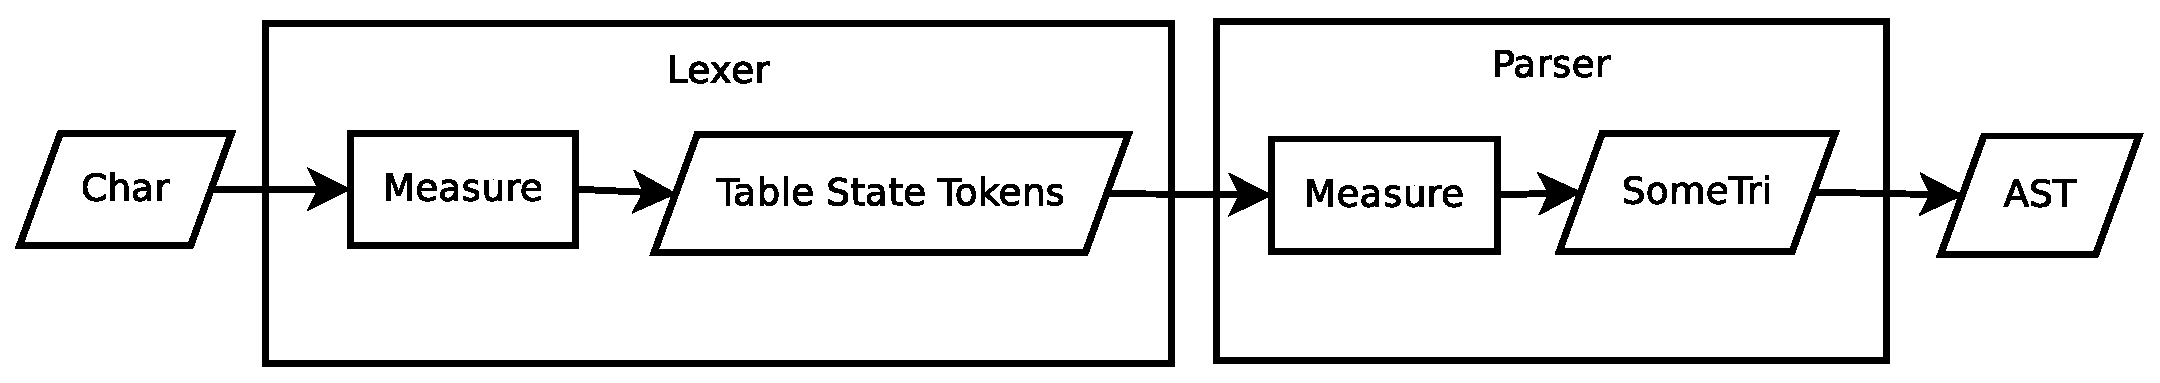
\includegraphics[width=\textwidth]{pipeline.eps}
\begin{code}
instance (Measured v IntToken) => Measured IntToken Char where
\end{code}
\caption{\label{pipelinedia}Diagram of measuring pipeline. The type signature
for the measured instance in the lexer shows the constraint: to measure a
\texttt{Char} into an \texttt{IntToken}, one has to be able to measure from
\texttt{IntToken} to some type \texttt{v}, which is defined as \texttt{SomeTri},
a type for upper-triangular matrices, in the parser.}
\end{figure}

We will describe what SomeTri is in more detail later, so for now it can be
thought of as the internal parser state. Looking at simple testing
code shows easily how the data progresses through the pipeline.
\texttt{stateToTree} is an auxiliary function extracting a \texttt{FingerTree}
from the internal lexer state.

\begin{figure}[H]
\begin{code}
test :: FilePath -> IO ([(CATEGORY,Any)])
test filename = do
    file <- readFile filename
    let lexed  = measure $ makeTree file
        parsed = measure $ stateToTree lexed
    return (results parsed)
\end{code} 
\caption{Code showing the measuring pipeline}
\end{figure}

Note that figure \ref{pipelinedia} is restricted to a single char. This process
is done for every char in the input source code, and the results are merged
using the monoid implementations of \texttt{mappend} for the lexer and the
parser. This behaviour is done internally in the finger tree with the call to
\texttt{measure}.  The lexer measure yields a lexer state containing tokens,
which are then in turn measured into the matrix type \texttt{SomeTri
[(CATEGORY,Any)]} by the parser, where each tuple holds a value of the
\texttt{CATEGORY} type, representing an intermediate parser state, such as an
almost-complete function header, and \texttt{Any} is a universal type that can
hold any value, and is used as an intermediary for the generated AST. 

The \texttt{Measured} instance for the lexer was written as part of the LexGen
project, and was only slightly modified to fit the parser. The \texttt{Measured}
instance for the parser is far more interesting, though. We can see how it works
in figure \ref{parsemeasure}.

\begin{figure}[H]
\begin{code}
instance Measured (SomeTri [(CATEGORY,Any)]) IntToken where
    -- Note: place the token just above the diagonal
    measure tok = T (bin' Leaf' Leaf') (q True :/: q False)
      where q b = quad Zero (t b) Zero Zero
            select b = if b then leftOf else rightOf
            t b = case intToToken tok of
                Nothing    -> Zero
                Just token -> One $ select b $ tokenToCats b token

\end{code}
\caption{\label{parsemeasure} Measure from token to upper-triangular matrix. The
\texttt{T} construct guarantees a square matrix of a given size. The call to
\texttt{quad} makes sure the observation about empty matrices by
\citet{parparsepaper} is handled properly when creating a matrix.}
\end{figure}

We create a 2x2 matrix, and place the lexed token in the upper-right corner
-- just above the diagonal. If the lexer did not return a token, a zero matrix
of the same size is created. This is shown in figure \ref{measurematrix}. In the
zero case, the call to \texttt{quad} enables the optimisation for empty matrices
by pattern matching and possibly choosing another matrix constructor (all
constructors are shown in figure \ref{mat} later).

\begin{figure}[H]
\centering
\begin{subfigure}[H]{.4\textwidth}
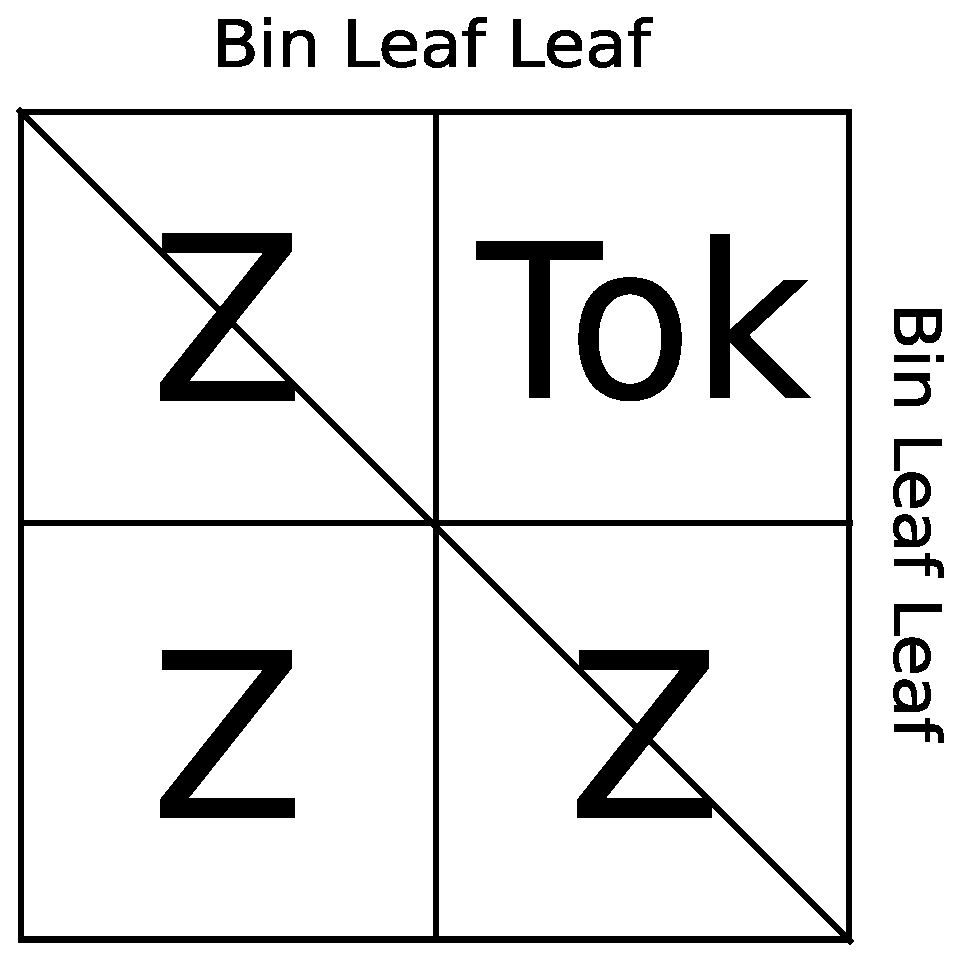
\includegraphics[width=.9\textwidth]{matrix2x2-token.eps}
\caption{2x2 matrix with a token}
\end{subfigure}
\begin{subfigure}[H]{.4\textwidth}
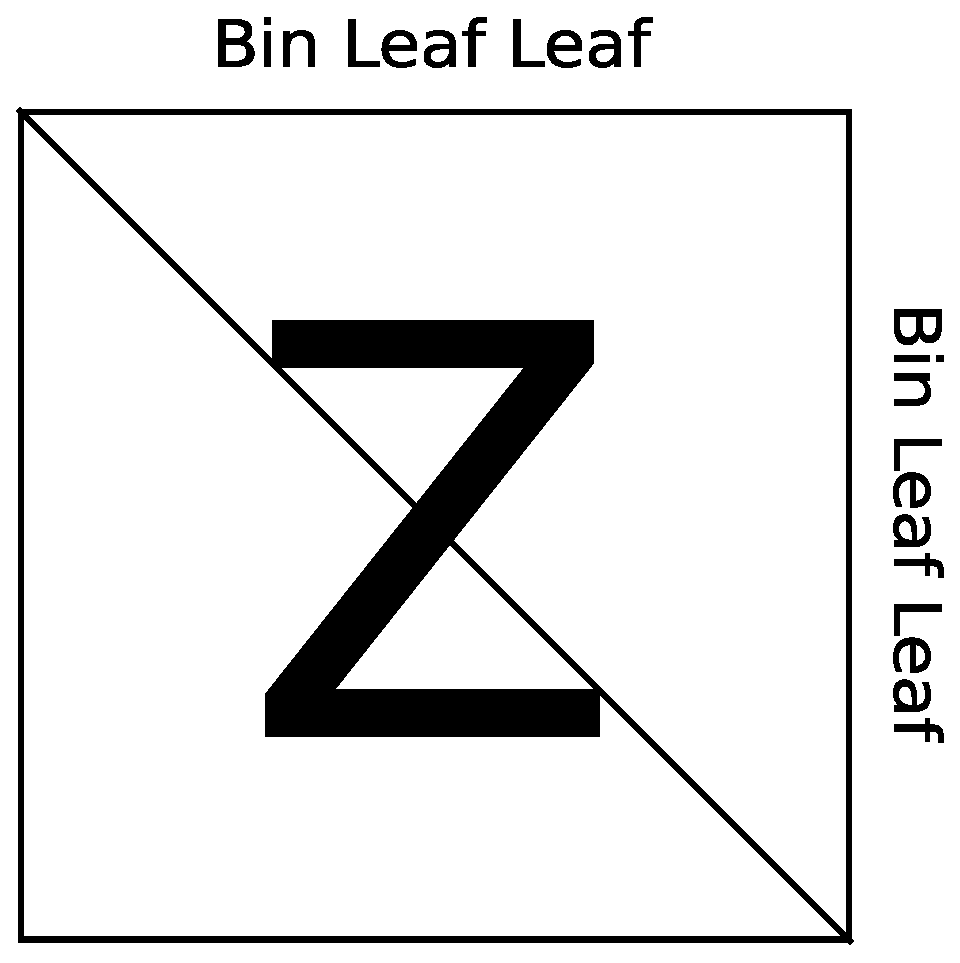
\includegraphics[width=.9\textwidth]{matrix2x2-zero.eps}
\caption{2x2 matrix without a token}
\end{subfigure}
\caption{\label{measurematrix} Graphical representation of the two possible
cases for measuring to matrices in the parser. Tok represents the set of all
rules $A$ such that $A ::= tok$ where tok is the lexed token.}
\end{figure}

Finally, the actual parsing happens in the \texttt{Monoid} instance for
\texttt{SomeTri}, where the call to merge in turn creates a call to
\texttt{closeDisjointP}, which in turn uses \texttt{mul}. The \texttt{mul}
function is defined in the typeclass \texttt{RingP}, our instance uses the
combine tables generated by the reference implementation in BNFC.

\begin{figure}[H]
\begin{code}
instance RingP a => Monoid (SomeTri a) where
    mempty = T Leaf' (Zero :/: Zero)
    t0 `mappend` t1 = unsafePerformIO $ do
      b <- randomIO
      return (merge b t0 t1)

instance RingP [(CATEGORY,Any)] where
  mul p a b = trav [map (app tx ty) l :/: map (app tx ty) r 
                   | (x,tx) <- a, (y,ty) <- b
                   , let l:/:r = combine p x y]
    where trav :: [Pair [a]] -> Pair [a]
          trav [] = pure []
          trav (x:xs) = (++) <$> x <*> trav xs
          app tx ty (z,f)  = (z, f tx ty)
\end{code}
\caption{\label{parsemonoid}Monoid instance for SomeTri, and RingP instance for
the parser data}
\end{figure}
The call to combine in figure \ref{parsemonoid} is the programming version of
checking if there exists a rule on the form $A ::= BC$ in the grammar.

\begin{figure}[H]
\centering
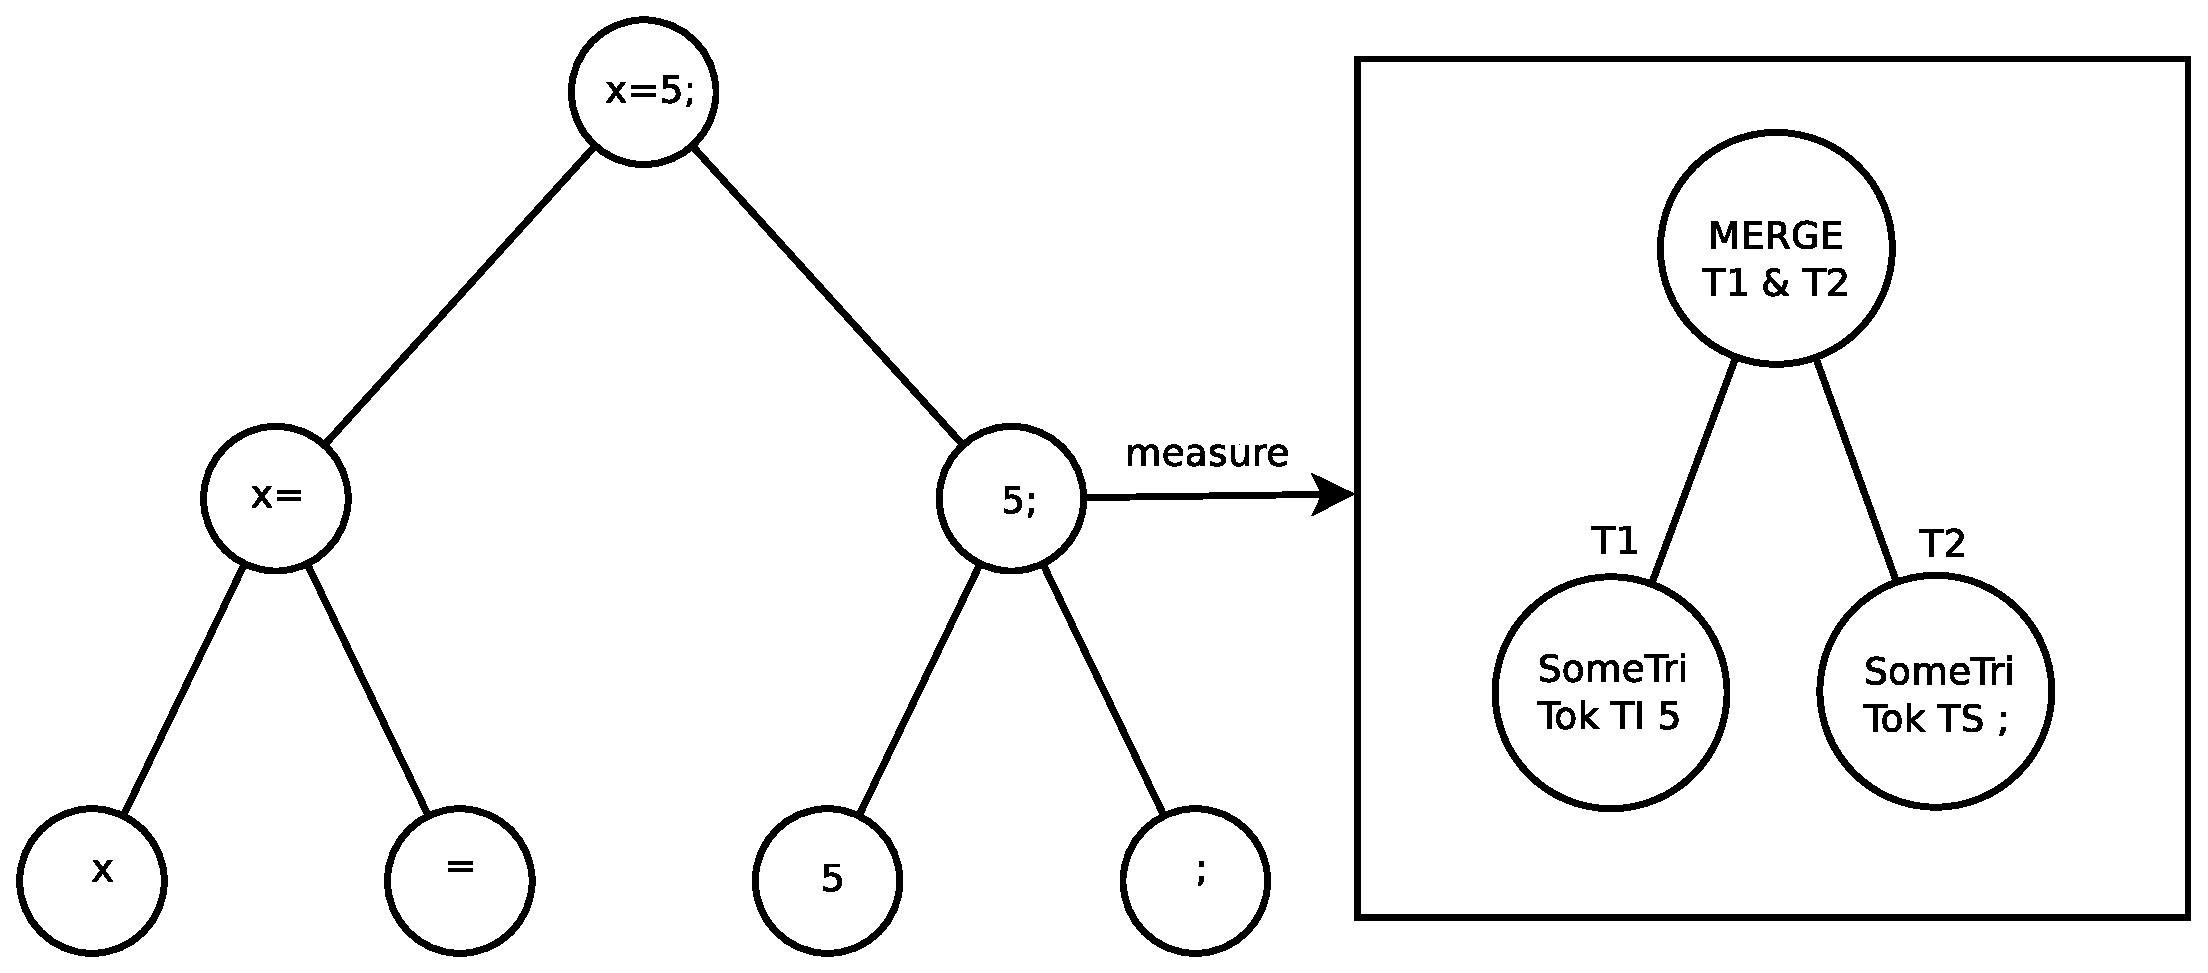
\includegraphics[width=.5\textwidth]{tree.eps}
\caption{\label{treemeasure}Graphical representation of lexing and parsing using
trees, with the measured parts enclosed in rectangles. Note that this is still a
simplification, all calls to \texttt{mappend} are not neccessary in order to
move forward in the process, and it is indeed possible to get an AST from just
one character by just measuring at one leaf, as shown in figure
\ref{pipelinedia}.}
\end{figure}

\subsection{Dependently typed programming with charts}
When merging the matrices, combining elements to create new, larger matrices, it
is important to keep the sizes of these matrices correct to avoid bugs that
would be hard to catch otherwise. The way this is done in the library available
in BNFC is by using dependent types. The existing code for merging could not be
used, but had to be extended to work in the tree/monoid setting. More on this
later.
% TODO: Referens till repo-forken.

First, the matrix type \texttt{Mat} is dependent on another type,
\texttt{Shape}, that describes the shape of a matrix as a binary tree.

\begin{figure}[H]
\begin{code}
data Shape = Bin Shape Shape | Leaf

data Mat :: Shape -> Shape -> * -> * where
  Quad :: !(Mat x1 y1 a) -> !(Mat x2 y1 a) ->
          !(Mat x1 y2 a) -> !(Mat x2 y2 a) ->
          Mat (Bin x1 x2) (Bin y1 y2) a
  Zero :: Mat x y a
  One :: !a -> Mat Leaf Leaf a
  Row :: Mat x1 Leaf a -> Mat x2 Leaf a -> Mat (Bin x1 x2) Leaf a
  Col :: Mat Leaf y1 a -> Mat Leaf y2 a -> Mat Leaf (Bin y1 y2) a
\end{code}
\caption{\label{mat}The \texttt{Mat} type with its dependent \texttt{Shape}
type. Note that shapes are used both for x- and y-axis size}
\end{figure}

Here are some example matrices, just to get a feel for how they are constructed.
\begin{figure}[H]
\begin{subfigure}[H]{.3\textwidth}
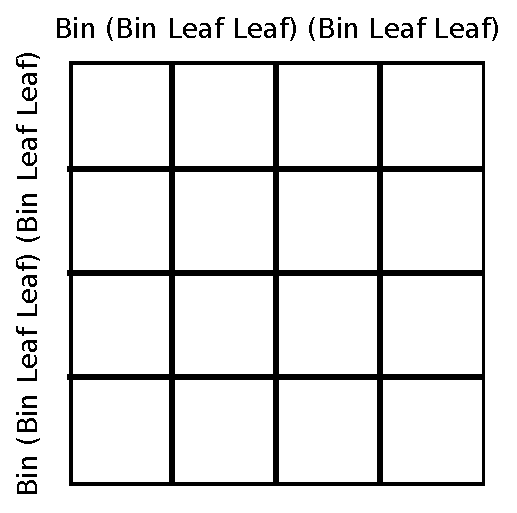
\includegraphics[width=120pt]{example-matrix-4x4.eps}
\caption{\texttt{Quad q1 q2 q3 q4} where q1-q4 are \texttt{Quad a b c d}} 
\end{subfigure}
\hfill
\begin{subfigure}[H]{.3\textwidth}
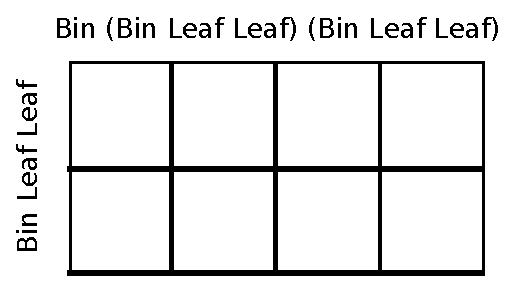
\includegraphics[width=120pt]{example-matrix-2x4.eps}
\caption{\texttt{Quad r1 r2 r3 r4} where r1-r4 are \texttt{Row a b}}
\end{subfigure}
\hfill
\begin{subfigure}[H]{.3\textwidth}
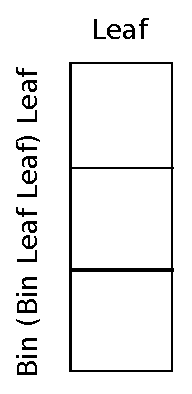
\includegraphics[height=120pt]{example-matrix-3x1.eps}
\caption{\texttt{Col (Col a b) c)}}
\end{subfigure}
\caption{Example matrices with their \texttt{Shape}s written out, and the
\texttt{Mat} constructor used to create them}
% TODO: Colour-code as suggested by solarus
% TODO: Fix the damn lines better

\end{figure}

In a setting without using finger trees and monoids, such as the reference
implementation by \citet{parparsepaper}, where this was implemented as
the \texttt{mergein} function, it is possible to merge matrices using a single
element as glue. Such an approach simplifies the merging a lot, because elements
are placed just above the diagonal and that means a single element can fill the
small void in the merged matrix, as illustrated in figure \ref{mergein}.

\begin{figure}[H]
\centering
\begin{subfigure}[H]{.45\textwidth}
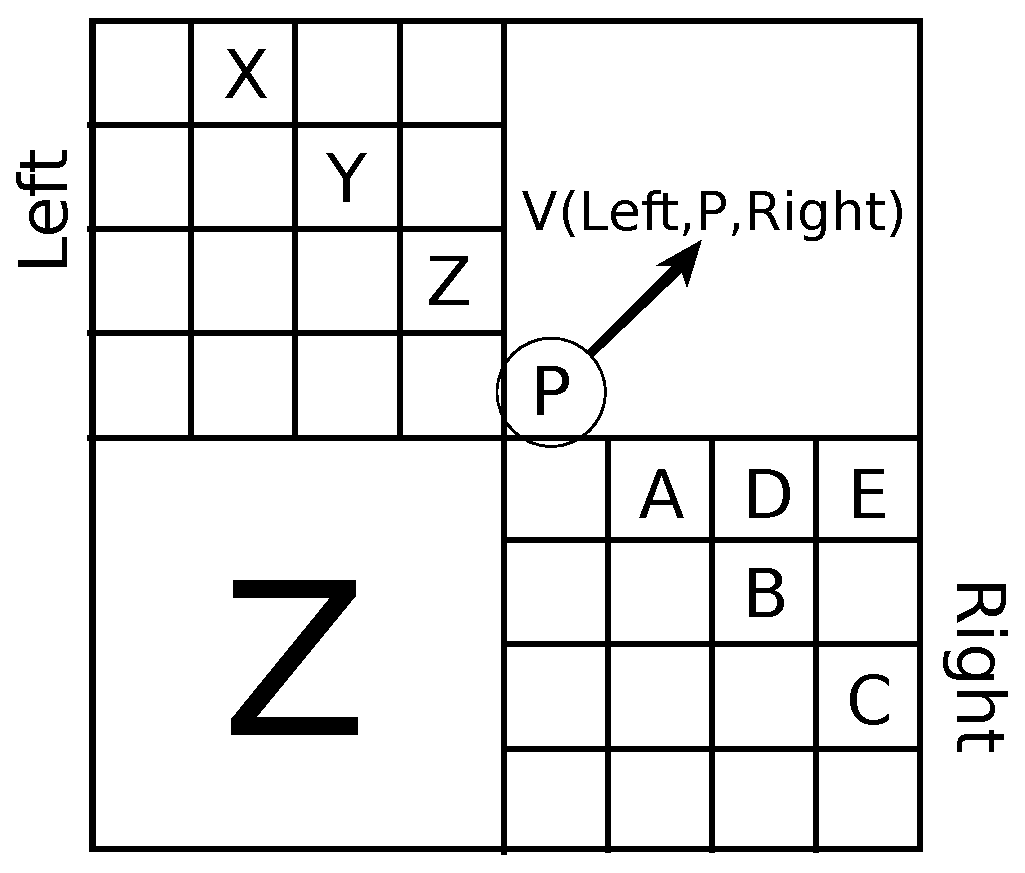
\includegraphics[width=.9\textwidth]{merge-with-element.eps}
\caption{Merging with middle element, as done by \citet{parparsepaper}}
\end{subfigure}
\hfill
\begin{subfigure}[H]{.45\textwidth}
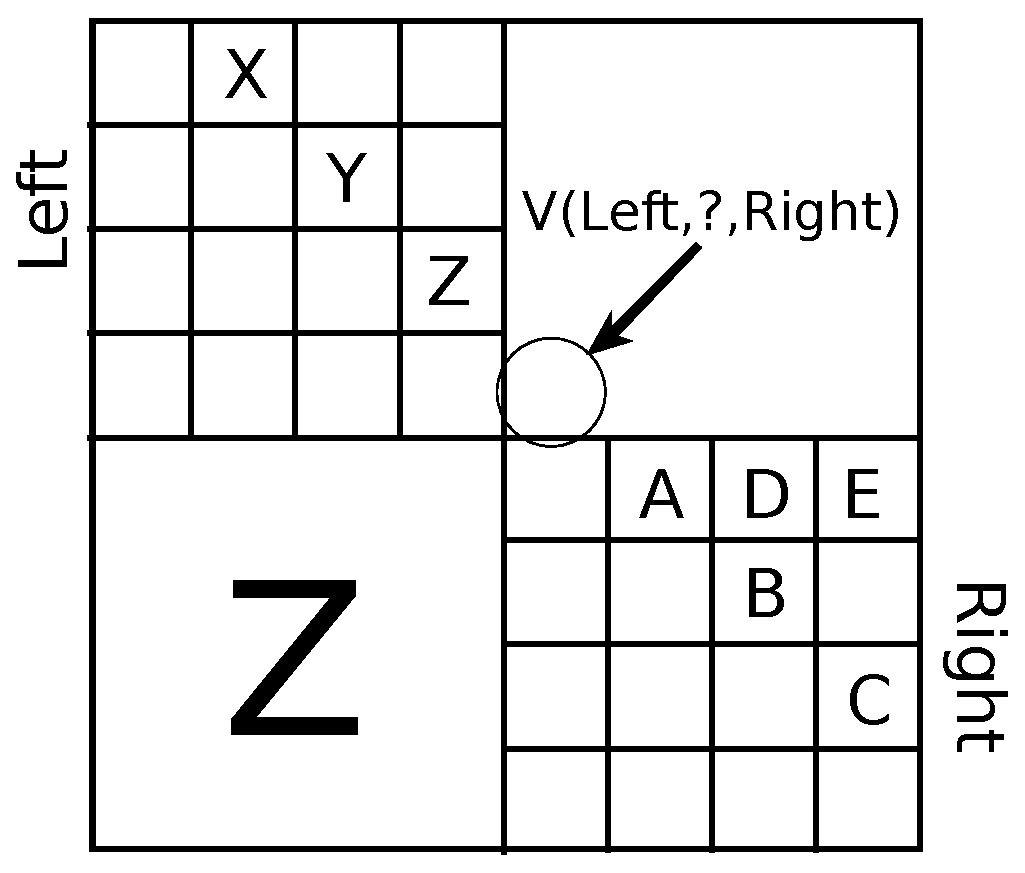
\includegraphics[width=.9\textwidth]{merge-without-element.eps}
\caption{Merge without middle element}
\end{subfigure}
\caption{\label{mergein}Merging with and without a single element as glue.
Without an element the diagonal is broken -- we cannot continue!}
\end{figure}

Because of the absence of an extra element, the existing function
\texttt{mergein} could not be used, but a merge function had to be implemented.
Without the extra element, the diagonal would be broken, and the algorithm would
not be able to move forward. We thus want to imitate the behaviour of having a
middle element.  The solution: chop off the first row in the second argument,
and recompute all but the leftmost elements when applying V. \label{chopsection}

\begin{figure}
\centering
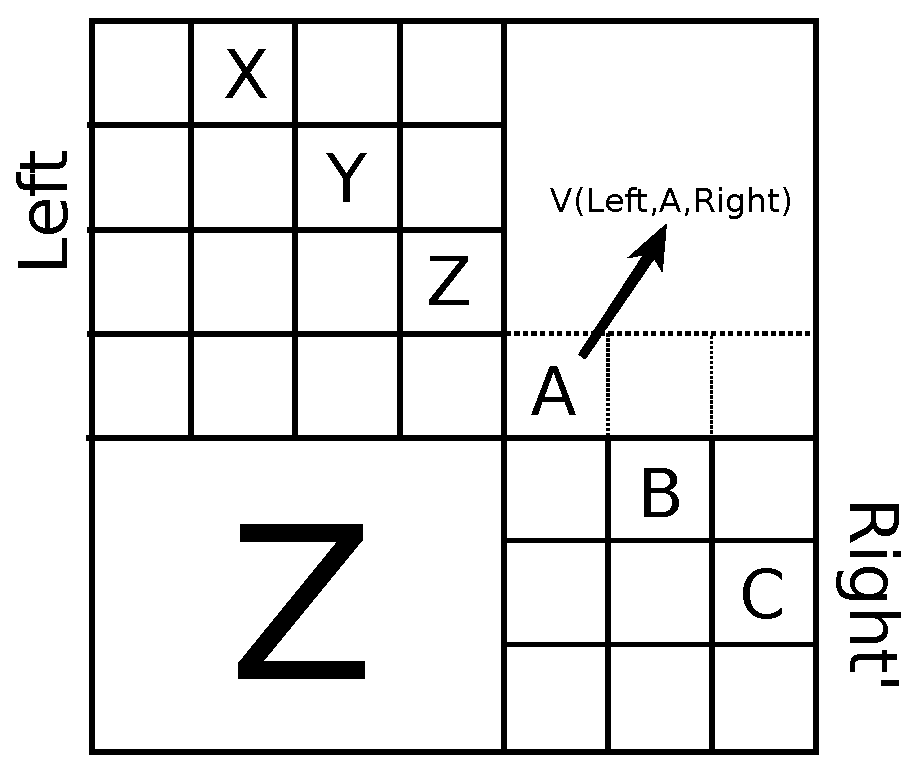
\includegraphics[width=.5\textwidth]{merge-with-chopping.eps}
\caption{\label{chopmerge}Successful merge without a middle element. The first
row on the right matrix is chopped off, we discard elements D and E and put A in
the leftmost bottom position, placing it just above the diagonal as wanted.}
\end{figure}

Before looking at the actual merge code, we should look at how the chopping
works. By pattern matching on the \texttt{Shape} in our \texttt{SomeTri} we can
get a data structure where the relation between a larger and smaller matrix can
be expressed. This data structure is \texttt{ChopFirst}. Once we obtain such a
value, we can pattern match on it to control our recursion for chopping, and
thus being able to give some guarantees about both the chopped matrix, and the
row that was chopped. This can be seen in figure \ref{chopfirst}.

\begin{figure}[H]
\begin{code}
data ChopFirst x x' where
  Stop :: ChopFirst (Bin Leaf x) x
  Continue :: ChopFirst x x' -> ChopFirst (Bin x x0) (Bin x' x0)

chopFirst :: ChopFirst x x' -> Mat x x a  
                            -> (Mat x' Leaf a, Mat x' x' a)
chopFirst _ Zero = (Zero,Zero)
chopFirst Stop (Quad a b c d) = (b,d)
chopFirst (Continue q) (Quad a b c d) =
  let  (e, a') = chopFirst q a
       (b',f)  = chopFirstRow q b
  in (row e f,quad a' b' zero d)
\end{code}
\caption{\label{chopfirst} The \texttt{ChopFirst} type and corresponding
function. Note that \texttt{chopFirst} discardes the first column of the matrix, as seen
in the \texttt{Stop} case}
\end{figure}

Note that \texttt{chopFirst}, as seen in figure \ref{chopfirst} does not match
the \texttt{Col}, \texttt{Row} or \texttt{One} constructors. For the
\texttt{One} case it is quite obvious because we cannot chop a 1x1 matrix. For
the other two, this is due to the type of \texttt{chopFirst}, where the input is
a square matrix: \texttt{Mat x x a}. Because both \texttt{Col} and \texttt{Row}
cannot be square (unless they're 1x1, in which case the \texttt{One} construct
should be used instead, which cannot be chopped anyway), there is no need to
check for them, and actually writing those cases would trigger a type error when
compiling.

Finally, before calling the function corresponding to the V function from
Valiant's algorithm, we need to \textbf{1)} throw away all but one value from
the chopped off row, and \textbf{2)} extend the row to match the size of the
matrices we merge with. This is done by a function called \texttt{mkLast'},
shown in figure \ref{mklast}.

\begin{figure}[H]
\begin{code}
mkLast' :: RingP a => Shape' y -> Mat x Leaf a -> Mat x y a
mkLast' Leaf' m = m
mkLast' (Bin' _ _ y) Zero = zero
mkLast' (Bin' _ _ y) (One a) = col zero (mkLast' y (one a))
mkLast' (Bin' _ _ y) (Row a b) = quad zero zero (mkLast' y a) zero
\end{code}
\caption{\label{mklast}Implementation of the mkLast function}
\end{figure}

We now have everything we need to create a new, larger, better matrix containing
soon-to-be abstract syntax trees. The code for \texttt{merge} is included in
figure \ref{merge}, resulting in a new quad, where the left matrix is left
untouched (as seen in figure \ref{chopmerge}), but we get a new, smaller, right
matrix, and the top-right part is computed using Valiant's algorithm. As usual,
all values below the diagonal are zero.

\begin{figure}[H]
\begin{code}
merge :: Bool -> SomeTri a -> SomeTri a -> SomeTri a
merge p (T y l) (T x r) = chopShape x $ \chopper x' ->
    let (rTopL, rL') = chopFirst chopper (leftOf r)
        (rTopR, rR') = chopFirst chopper (rightOf r)
        cdp = closeDisjointP p (leftOf l) 
                (mkLast' y $ sequenceA (rTopL :/: rTopR)) rR'
    in T (bin' y x') (quad' l cdp zero (rL' :/: rR'))
\end{code}
\caption{The function \texttt{merge} without middle element}
\label{merge}
\end{figure}

\subsection{Oracle and unsafePerformIO}
\label{oraclesection}
The use of an oracle as described by \citet{parparsepaper} presented a bit
of a problem in implementing a monoid instance for the parser, for the simple
reason that it is very hard to simply pick a boolean value at random in Haskell
without it being always \texttt{True} or always \texttt{False}. The call to
\texttt{merge} in \texttt{mappend} illustrates this clearly:

\begin{figure}[H]
\begin{code}
instance Monoid (SomeTri a) where
    t0 `mappend` t1 = merge True t0 t1
\end{code}
\caption{First attempt at parser Monoid instance before random oracle.}
\end{figure}

The call to \texttt{merge} requires a \texttt{Bool} acting as the oracle as an
argument. Because a Monoid has no context outside its own type, it is hard, if not
impossible, to generate a \texttt{Bool} using only the \texttt{SomeTri} type.
One could argue for creating a newtype wrapper around a tuple of
\texttt{SomeTri} and \texttt{StdGen}, used to generate the \texttt{Bool} at each
step, but that only moves the problem to the \texttt{mempty}
call, where a fresh \texttt{StdGen} would have to be picked at each instance.

The solution to this problem came in the form of a call to
\texttt{unsafePerformIO}.  Not only is this is controversial, it was also not
completely obvious to implement. If an unsafe call to \texttt{randomIO} was made
separately from the merge call, this call would be evaluated only once,
rendering the solution useless. The trick here was to put the whole call inside
an unsafe wrapper, so that the call to merge, and with that the call to
\texttt{randomIO}, became dependent on the input.

\begin{figure}[H]
\begin{code}
instance Monoid (SomeTri a) where
    t0 `mappend` t1 = unsafePerformIO $ do
      b <- randomIO
      return $ merge b t0 t1
\end{code}
\caption{Parser \texttt{Monoid} instance with oracle}
\end{figure}

Now usually, for \texttt{unsafePerformIO} to be safe one should make sure that
the call is free from side effects and \textit{independent of its environment}.
\cite{unsafeHackage}. None of those two requirements are fulfilled here, so 
this calls for discussion. In general, one does not want a call to
\texttt{unsafePerformIO} to be evaluated more than once -- but in this case this
is a requirement for the code to behave as expected, and that's why it is indeed
dependent on its environment. The only side effect in this snippet is the use of
the global random number generator and that should not affect any other part of
the program, and can thus be considered safe.

%
% NEW CHAPTER
%

\chapter{Results}
We have managed to write a parser that is incremental and which, when given
correct input, produces correct output in the form of an AST. The parser, and
the accompanying lexer, can be generated by BNFC. When given incorrect input
however, the output is not especially satisfactory. The lexer can tell if an
incorrect token is part of the input, but it cannot tell where in the input that
token is placed. The parser can also recognise that the input tokens does not
follow the grammar of the language, but it cannot give any information about
where the syntactic error was made.

\section{Possible text editor setting}
TODO: Write something here that connects to the motivation

\section{Testing}
Being able to generate lexer and parser using BNFC, only needing a LBNF grammar
file, testing for different language was made easy. The main testing language
was Javalette Light, a small subset of C, but still with the ability to create
interesting parse trees. Later, both the Javalette language and C was used to
test the parser. When testing with C a serious bug was discovered, this is
discussed in \ref{branchbug}.

Testing was not automated, but instead simple input files were used, where the
source code was either correct or had some syntax error. This proved to be
sufficient for this project, but for future versions, when hand-written cases
might not be enough to cover all trivial uses, one would probably want to have
tests generated by something like quickcheck. Although one would probably get
quite far by being systematic and using the given grammar as a base for test
cases. 
% TODO: Cite quickcheck

\section{Measurements}
% TODO: Cite criterion
We have been using criterion as a benchmarking library to test the
implementation. Benchmarking included both measuring of the merge step with two
previously parsed subtrees as well as measuring the time to parse input of
increasing sizes. Most measuring was done on a computer running an Intel i7
processor clocked at 3.40 GHz, with a sample size of 1000. 

It should be noted that testing large inputs for this project has been hard due
to large memory consumption, possibly owing to the structure of the lexer.
Because not all tests look the same, this constraint affect different
measurements differently, so the same input sizes have not been possible to use
for the merge test and the more general running time test.

\subsection{Behaviour}
The input to the parser is a fingertree, generated by the lexer. We will ignore
the behaviour of the lexer, because it is not the main scope of this project, but
instead look a bit about how the parser should behave when it comes to time
complexity. The steps taken to parse the input is to first create the initial
matrix at each leaf. The time at each leaf is independent on the input size, and
is therefore $O(1)$, but it is done at each leaf, se the total is $O(n)$. The
second step is the merging, which at each point also does the matrix
multiplications -- shown by \citet{parparsepaper} to be $O(log^3 n)$.
Implementation of the merging step was relatively straight-forward, and should
therefore satisfy these conditions. 

\subsection{Merging matrices}
The core of the parser is the merging of matrices corresponding to previously
parsed subtrees. This should be fast, and not depend on the input size at all.
It turns out that it is indeed independent of input size, and the merge function
is almost constant in time with respect to the size of the subtrees.

\subsection{Total running time}
From stress testing the parser with large inputs, it seems that the parser
behaves as expected relative to the input size, growing in a linear fashion with
it, corresponding well to the expected behaviour.

\begin{figure}[H]
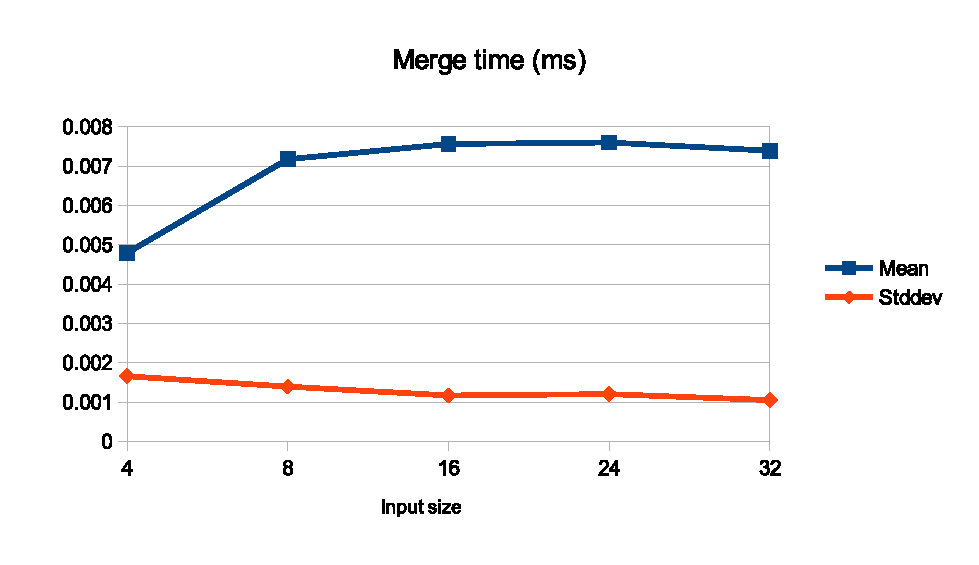
\includegraphics[width=\textwidth]{criterion-merge.eps}
\caption{\label{critmerge}Merge times for files where the input size denote the
number of functions (of equal size) in that file.}
\end{figure}

\begin{figure}[H]
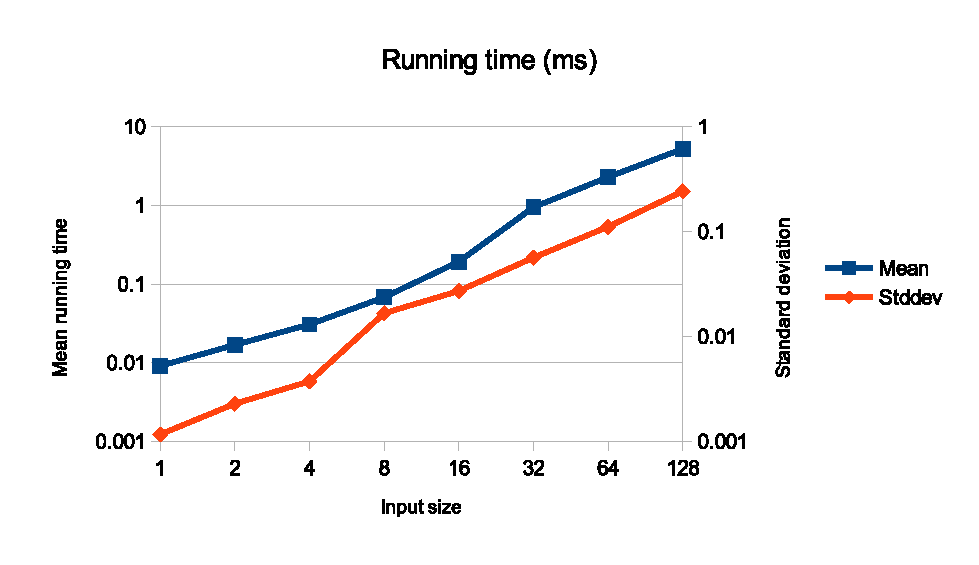
\includegraphics[width=\textwidth]{criterion-1-128.eps}
\caption{\label{criterion}Running time for files where the input size denote the
number of functions (of equal size) in that file. Note that a logarithmic scale
is used on both axes.}
\end{figure}

%
% NEW CHAPTER
%
\chapter{Discussion}
% TODO: Write introduction here

\section{Pitfalls}
During implementation, a few mistakes that are worth mentioning was made. These
are discussed here. There were of course more than these, but most of them were
reasonably small, and were not theoretically difficult to solve, but rather
straight-forward implementation bugs. 

\subsection{Too many parse results}
When the parser was finally working, there was an issue that, whenever a file
was successfully parsed, the parser returned a number of results, from 4 to
1024, all identical to each other. This led us to believe that there was
branching done in places where no branching was motivated. It turned out to be
due to a bug in \texttt{merge}, in the subroutine taking care of the row that
was chopped (see \ref{chopsection}). Initially, \texttt{merge} was written so
that the chopped off row was included as a part of the upper-right matrix as an
argument to the V function. This led that row to be combined with itself,
because that row had already been computed using the V function. The solution
was to remove all but the first element, so that nothing would be recomputed.

Another bug, similar to the one described above, was discovered late in the
project and has thus not been investigated as much. The results are the same --
too many parse results, but they are always the same number, and depend on
certain constructs in the input source code. Due to time constraint it has not
been possible to pinpoint the source of this bug, but the behaviour suggests an
error in \texttt{merge}. \label{branchbug}

\subsection{Loosen constraint on Matrix type}
When writing \texttt{merge}, one attempt was made at loosening the constraints
on the \texttt{Row} and \texttt{Col} constructors so that they could correspond
to more than one row or col, respectively. This turned out to be a bad idea when
one wanted to control recursion using these constructors. Such a change also
introduced an ambiguity in the semantics of matrices, because then a 4x4 matrix
could be created by using \texttt{Quad} (the right way), or by using the less
strict versions of \texttt{Col} (a wide column of height four) or \texttt{Row}
(a tall row of width four). Having the different constructors constrained to a
certain type of matrix proved easier in the end, and the extra work in terms of
pattern matching was worth it to avoid the extra work needed every time a
\texttt{Row} or \texttt{Col} was encountered -- just to check their height and
width, respectively.  

\section{Future work}
The result of this project is a parser that can parse correct input and does
that well. There are two main features missing however; position information on
tokens, and good error reporting.

\subsection{Position information}
Position information for tokens is a feature that is currently missing in the
parser, much due to the fact that it is missing in the lexer. Discussions with
Hannson \& Hugo revealed that this is due to that not being a priority. The
most likely way to implement position information would be by using relative
positions for tokens, because of the tree structure where nodes are not aware of
each other. That way, position information, or lexical errors, can be promoted
using mappend. There are, however, several ways to integrate the relative
positions into the structure, but the most obvious would be to create a newtype
wrapper for tuples where the lexer state and position information are dependent
on each other, as opposed to the monoid instance for regular tuples. 

\subsection{Error information}
Related to the issue of position information, the error reporting in the lexer
and parser is poor to say the least. Invalid tokens are reported by the lexer,
but invalid syntax is only reported by saying that there were more than one
parse result. For the lexer, the only thing missing in error reporting is
said position information. This is, of course, true for the parser as well, but
due to the structure of the parser it is harder to know where an error was made.

The reason for why it is hard to know where an error was made owes to the matrix
structure and how rules are combined as $A ::= BC$. Using the CYK algorithm, it
would be possible to have overlaps in the parse results (where one would have to
choose one to move further, as shown in figure \ref{parseoverlap}), and an error
in the middle of a code snippet could lead to the parsing resulting in many
small results that lack structural \textit{glue}, as shown in figure
\ref{missingglue}. 

\begin{figure}[H]
  \centering
  \begin{subfigure}[H]{.4\textwidth}
    \flushleft
     \begin{tikzpicture}
       \pgftransformrotate{-90}
       \pgftransformscale{0.5}
       \draw (0,0) -- (10,10);
       \subt 0 2 {$A$};
       \subt 2 4 {$B$};
       \subt 0 4 {$C$};
       \subt 5 7 {$X$};
       \subt 7 9 {$Y$};
       \subt 5 9 {$Z$};
       \mrk 4 {$j$};
       \mrk 5 {$k$};
     \end{tikzpicture}
     \caption{\label{missingglue}Example chart where the tokens from j to k
     cannot be parsed, and therefore $C$ and $Z$ are given as parse results.}
  \end{subfigure}
  \begin{subfigure}[H]{.1\textwidth}
  \text{}
  \end{subfigure}
  \begin{subfigure}[H]{.4\textwidth}
    \flushright
    \begin{tikzpicture}
      \pgftransformrotate{-90}
      \pgftransformscale{0.5}
      \draw (0,0) -- (10,10);
      \subt 2 6 {$A$};
      \subt 4 8 {$B$};
      \mrk 2 {$j$};
      \mrk 8 {$k$};
    \end{tikzpicture}
    \caption{\label{parseoverlap} Example chart where $A$ and $B$ overlap. Here one
    has to decide on how to proceed if there is no rule that can parse from j to
    k.}
  \end{subfigure}
\end{figure}

%
% BIBLIOGRAPHY
%

\bibliographystyle{plainnat}
\bibliography{bibliography}

%
% ANY APPENDICES HERE
%

\appendix
\chapter{Javalette Light}

% TODO: Use the REAL javalette light grammar that was used in the project
\section{LBNF grammar}
\begin{code}
Prog.     Prog     ::= [Fun];
Fun.      Fun      ::= Typ Ident "(" ")"  [Stm] ;

SDecl.    Stm      ::= Typ Ident ";"  ;
SAss.     Stm      ::= Ident "=" Exp ";"  ;
SIncr.    Stm      ::= Ident "++" ";"  ;
SWhile.   Stm      ::= "while" "(" Exp ")" [Stm]  ;

ELt.      Exp      ::= Exp1 "<" Exp1 ;
EPlus.    Exp1     ::= Exp1 "+" Exp2 ;
ETimes.   Exp2     ::= Exp2 "*" Exp3 ;
EVar.     Exp3     ::= Ident ;
EInt.     Exp3     ::= Integer ;
EDouble.  Exp3     ::= Double ;

_.        Stm      ::= Stm ";" ;
coercions Exp 3 ;

TInt.     Typ  ::= "int" ;
TDouble.  Typ  ::= "double" ;
\end{code}

\newpage
\section{Sample code}
\begin{code}
int main() {
    int p;
    int x;
    x = 2;
    p = 2;
    while(p < 5) {
        x = x * x;
        p++;
    }
}
\end{code}


\end{document}
